\documentclass[12pt]{article}
\usepackage[english]{babel}
\usepackage[utf8x]{inputenc}
\usepackage{amsmath}
\usepackage{graphicx}
\graphicspath{{Images/}}
\usepackage[colorinlistoftodos]{todonotes}
\usepackage{listings}
\usepackage{hyperref}
\usepackage{float}
\usepackage{tikz}
\usetikzlibrary{positioning,fit,arrows.meta,backgrounds}
\graphicspath{ {images/} }


\usepackage{xcolor}

\definecolor{codegreen}{rgb}{0,0.6,0}
\definecolor{codegray}{rgb}{0.5,0.5,0.5}
\definecolor{codepurple}{rgb}{0.58,0,0.82}
\definecolor{backcolour}{rgb}{0.95,0.95,0.92}

\lstdefinestyle{mystyle}{
	backgroundcolor=\color{backcolour},   
	commentstyle=\color{codegreen},
	keywordstyle=\color{magenta},
	numberstyle=\tiny\color{codegray},
	stringstyle=\color{codepurple},
	basicstyle=\ttfamily\footnotesize,
	breakatwhitespace=false,         
	breaklines=true,                 
	captionpos=b,                    
	keepspaces=true,                 
	numbers=left,                    
	numbersep=5pt,                  
	showspaces=false,                
	showstringspaces=false,
	showtabs=false,                  
	tabsize=2
}

\lstset{style=mystyle}
\setcounter{tocdepth}{4}
\setcounter{secnumdepth}{4}

\tikzset{
	module/.style={%
		draw, rounded corners,
		minimum width=#1,
		minimum height=5mm,
		font=\sffamily
	},
	module/.default=2cm,
	>=LaTeX
}


\begin{document}
	\begin{titlepage}
		\newcommand{\HRule}{\rule{\linewidth}{0.1mm}} 
		\center 
		\includegraphics[scale=0.12]{ceng.jpg} \\
		\vspace{1cm}
		\textsc{\Large MIDDLE EAST TECHNICAL UNIVERSITY}\\[0.5cm]
		\textsc{\large Department Of Computer Engineering}\\[0.5cm]
		\textsc{\large CENG 300}\\
		\HRule \\[0.4cm]
		{ \huge \Large Summer Practice Report }\\[0.4cm]
		METU Data Mining Research Group \\
		Start Date: \hspace{25px}  End Date: \\
		Total Working Dates:
		
		\HRule \\[0.3cm]
		{\today}\\[1.2cm]
		
		
		\begin{minipage}{0.4\textwidth}
			\begin{flushleft} \large
				
				\emph{Student:}\\
				Onat ÖZDEMİR
			\end{flushleft}
			
			
		\end{minipage}
		\begin{minipage}{0.4\textwidth}
			\begin{flushright} \large
				\emph{Instructors:} \\
				Prof.Dr.Pınar KARAGÖZ \\
			\end{flushright}
			\begin{flushright} \large
				Prof.Dr.İsmail Hakkı TOROSLU \\
			\end{flushright}
		\end{minipage}\\[1cm]
		\vspace{2cm}
		
		
		Student's Signature \hspace{150px} Organization Approval \\
		
		
	\end{titlepage}
	
	\include{GradingRubric}
	\tableofcontents          
	\newpage
	
	\section{Introduction}
	I have done my summer internship at METU Data Mining Research Group under the supervision of Prof.Dr.Pınar KARAGÖZ and Prof.Dr.İsmail Hakkı TOROSLU. The task I have worked on was implementing a Trust Based Recommender using the collaborative filtering method and testing it on provided dataset. The dataset contains information about customers and the products they have bought. In addition to dataset, I was able to use eigentrust calculation and community detection modules provided by the TACOREC.
	
	\section{Project}
	During the internship, I implemented two trust based recommenders with different weightening methods:
	\begin{enumerate}
		\item Eigentrust Weighted Recommender
		\item Inverse Distance Weighted Recommender
	\end{enumerate} 
	The details of these two recommenders can be found in section 2.4 and 2.5, respectively.
	
	\subsection{Analysis Phase}
	There were two problems I need to solve: \\
	1 - Dataset was very sparse \\ 
	2 - There was no explicit trust information \\
	In the both implementations I have made, first case handled by filtering the customers and products which purchased and were bought more than filtering threshold times. To gain better understanding on the second problem, I studied implicit trust calculation methods and looked into lots of research papers.
	
	\subsection{Design Phase}
	\subsection{Implementation Phase}
	Since there are two different implementations, I have divided the implementational details of the recommenders into two subsections: section 2.4 and 2.5. Under this subsection, libraries and technologies used in implementations are explained.
	\subsubsection{Neo4j}
	\subparagraph{Driver Installation}:
	\begin{lstlisting}[language=bash]
	pip install neo4j
	\end{lstlisting}
	
	\subparagraph{Configuration}:
	\begin{lstlisting}[language=python]
	import neo4j
	...
	
	uri = self._config["database"]["neo4j"]["uri"]
	user = self._config["database"]["neo4j"]["user"]
	password = self._config["database"]["neo4j"]["password"]
	
	self._driver = neo4j.Driver(uri, auth=(user, password))
	
	\end{lstlisting}
	
	\subparagraph{Sample Usage}:
	\begin{lstlisting}[language=python, caption=Neo4j driver example]
	import neo4j
	...
	
	def get_customer_trust(self, customer_id):
	
	query = (
	f"MATCH (u:Customer)-[r:BELONGS_IN]->(:Community) "
	f"WHERE u.id = {repr(customer_id)} "
	f"RETURN r.eigentrust"
	)
	
	with self._driver.session() as session:
	return tuple(session.run(query).single())
	
	\end{lstlisting}
	
	\subsubsection{Numpy}
	\subparagraph{Installation}:
	\begin{lstlisting}[language=bash]
	pip install numpy
	\end{lstlisting}
	
	\subparagraph{Sample Usage}:
	\begin{lstlisting}[language=python, caption=Numpy example]
	import numpy as np
	
	class TrustBasedFilterer(object):
	...
	
	def _create_customers_versus_products_table(self):
	
	self._customers_versus_products_table = np.zeros(
	(self._unique_customers.shape[0],
	self._unique_products.shape[0]),
	dtype=np.bool,
	)
	
	self._customers_versus_products_table[
	self._sales[:, 0],
	self._sales[:, 1],
	] = True
	\end{lstlisting}
	
	\subsubsection{Scipy}
	\subparagraph{Installation}:
	\begin{lstlisting}[language=bash]
	pip install scipy
	\end{lstlisting}
	
	\subparagraph{Sample Usage}:
	\begin{lstlisting}[language=python, caption=Scipy example]
	from scipy.sparse import csr_matrix
	from scipy.sparse.csgraph import dijkstra
	
	class Graph(object):
	...
	
	def _create_distance_matrix(self):
	
	self._create_adjacency_matrix()
	
	self._adjacency_matrix = \
	csr_matrix(self._adjacency_matrix)
	
	self._distance_matrix = dijkstra( 
	csgraph=self._adjacency_matrix, 
	directed=False, 
	return_predecessors=False, 
	unweighted=True,
	limit=self._max_distance)
	
	self._distance_matrix\ 
	[~np.isfinite(self._distance_matrix)] = 0
	\end{lstlisting}
	
	
	\subsection{Eigentrust Weighted Trust Based Recommender}
	\begin{figure}[H]
		\centering
		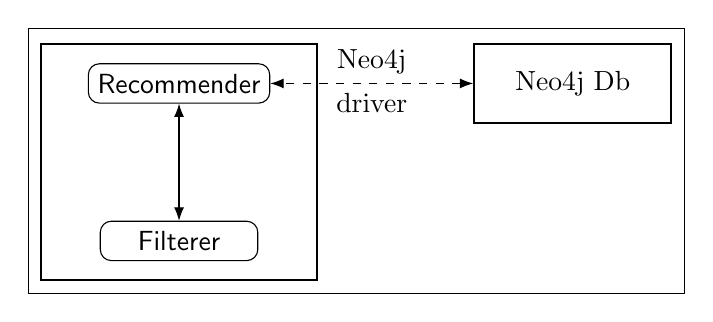
\begin{tikzpicture}[
		% This will show the frame around the figure
		show background rectangle]
		
		% Place first 6 items
		\node[module] (recommender) at (0,2) {Recommender};
		\node[module] (filterer) at (0,0) {Filterer};
		
		
		\node (fit) at (0,1) [draw,thick,minimum width=3.5cm,minimum height=3cm] {};
		
		\node (db) at (5,2) [draw,thick,minimum width=2.5cm,minimum height=1cm] {Neo4j Db};
		
		
		%arrow between boxes
		\draw[<->,dashed] (db)-- node[above] {Neo4j} node[below] {driver} ++ (recommender);
		
		\draw[<->] (recommender)--(filterer);
		
		\end{tikzpicture}
		\caption{Recommender Structure}
	\end{figure}
	\subsubsection{About Eigentrust}
	Eigentrust\cite{Eigentrust} is a reputation calculation algorithm mainly designed for peer-to-peer networks. In our case, Eigentrust represents how strongly connected the customers are to their communities. Eigentrust values calculated by the eigentrust module provided by TACoRec\cite{Tacorec} and stored in Neo4j database as a property of the relationship between a customer and his/her community. 
	\subparagraph{Problem encountered with Eigentrust:}
	Especially for the customers connected to communities with small size and low densities, eigentrust values stored in the database are either very small or equal to zero. Most of the customers with zero eigentrust values are eliminated after filtering the network from customers with a small number of products. Unfortunately, eigentrust values ​​are still quite small.
	
	\subsection{Inverse Distance Weighted Trust Based Recommender}
	\begin{figure}[H]
		\centering
		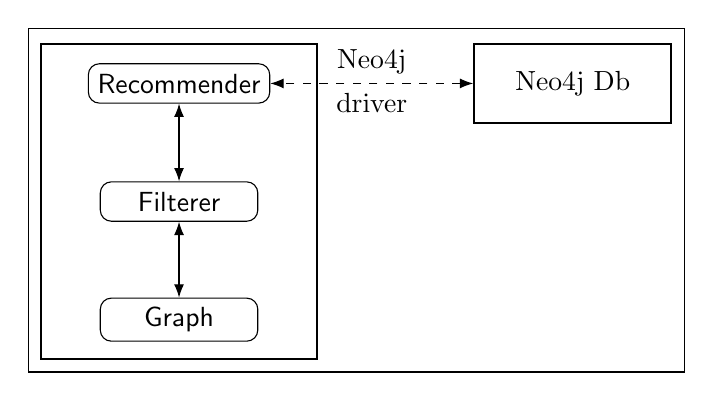
\begin{tikzpicture}[
		% This will show the frame around the figure
		show background rectangle]
		
		% Place first 6 items
		\node[module] (recommender) at (0,1.5) {Recommender};
		\node[module] (filterer) at (0,0) {Filterer};
		
		
		\node (fit) at (0,0) [draw,thick,minimum width=3.5cm,minimum height=4cm] {};
		
		\node (db) at (5,1.5) [draw,thick,minimum width=2.5cm,minimum height=1cm] {Neo4j Db};
		
		\node[module] (graph) at (0,-1.5) {Graph};
		
		%arrow between boxes
		\draw[<->,dashed] (db)-- node[above] {Neo4j} node[below] {driver} ++ (recommender);
		
		\draw[<->] (recommender)--(filterer);
		\draw[<->] (filterer)--(graph);
		
		\end{tikzpicture}
		\caption{Recommender Structure}
	\end{figure}
	Inverse Distance Weighted Trust Based Recommender consists of three modules:
	
	\subsubsection{Graph Module} Responsible for creating adjacency matrix from given customer versus product matrix, calculating the distances between customers applying djkstra algorithm to the adjacency matrix using scipy library, and calculating the trust by taking the recreciprocal of the distance matrix.
	\paragraph{Constructing Adjacency Matrix and Distance Matrix}\mbox{}\\
	To construct the "adjacency matrix" from customer versus products table, I propose two methods:
	\subparagraph{Proposed Method 1: Unweighted Graph}\mbox{}\\
	In this method, the "adjacency matrix" is constructed based on whether customers purchased a joint product or not. In other words, edge between two customers can exist if and only if the intersection of the set of products they purchased is not the empty set.
	\begin{figure}[H]
		\centering
		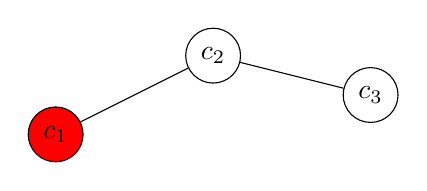
\begin{tikzpicture}
		\node[shape=circle,draw=black, fill = red] (a) at (0, 2)     {\textbf{$c_{1}$}};
		\node[shape=circle,draw=black] (b) at (2, 3)     {$c_{2}$};
		\node[shape=circle,draw=black] (c) at (4, 2.5)     {$c_{3}$};
		
		
		\path[-] (a) edge (b);
		\path[-] (b) edge (c);
		\end{tikzpicture} 
		\caption{$c_{1}$ and $c_{2}$ have purchased at least 1 joint product, but $c_{1}$ and $c_{3}$ do not have a joint product}
	\end{figure}
	
	\subparagraph{Proposed Method 2: Euclidean Distance Weighted Graph}\mbox{}\\
	In this method, the "adjacency matrix" is constructed based on the "euclidean distances"\ref{eqn:euclidean_distance} between customers. 
	\begin{equation} 
	\label{eqn:euclidean_distance}
	\begin{split}
	adj[c_{1}]][c_{2}] = \sqrt{\sum_{i\in I_{1}\cap I{2}}^{} (r1_{i}-r2_{i})^2}
	\end{split}
	\end{equation}
	where $r1_{i}$ and $r2_{i}$ represents ratings given by $c_{1}$ and $c_{2}$ for product $i$. Unlike the commonly used "euclidean distance" calculation, in this method, only ratings given to joint products are included in the calculation.
	\begin{figure}[H]
		\centering
		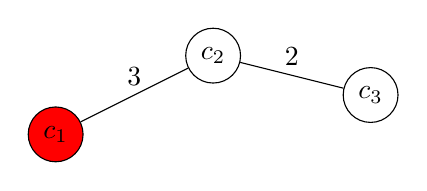
\begin{tikzpicture}
		\node[shape=circle,draw=black, fill = red] (a) at (0, 2)     {\textbf{$c_{1}$}};
		\node[shape=circle,draw=black] (b) at (2, 3)     {\textbf{$c_{2}$}};
		\node[shape=circle,draw=black] (c) at (4, 2.5)     {\textbf{$c_{3}$}};
		
		
		\path[-] (a) edge node[above]{3} (b);
		\path[-] (b) edge node[above]{2} (c);
		\end{tikzpicture} 
		\caption{euclidean distance between $c_{1}$ and $c_{2}$ equals 3, and $c_{1}$ and $c_{3}$ do not have a joint product}
	\end{figure}
	\textbf{Problem encountered with euclidean distance method:} As the module is generally tested on sparse datasets, 
	
	\subparagraph{Dijkstra's Algorithm}\mbox{}\\
	To construct the "distance matrix", the graph module uses "Dijkstra's Algorithm"\cite{Dijkstra} which takes the adjacency matrix as parameter and returns the distance matrix.
	
	\paragraph{Trust Calculation}\mbox{}\\
	After calculating the shortest distance between each pair of customers using "Dijkstra's Algorithm", to calculate the trust score between customers Graph module uses
	\begin{equation*} 
	T(c_{1}, c_{2})= \left\{
	\begin{array}{lr} 
	\frac{1}{d(c_{1}, c_{2})} & d(c_{1}, c_{2}) \neq np.inf \\
	0 & d(c_{1}, c_{2}) = np.inf
	\end{array}
	\right.
	\end{equation*}
	function where $d(c_{1}, c_{2})$ represents the shortest distance between the $customer_{1}$ and $customer_{2}$.
	
	\textbf{A benefit of the method:} Especially for excessively sparse datasets, recommenders using euclidean distance-based similarity fails since they cannot calculate similarity score for the the customer pairs with no common products.	Since the  "Dijkstra's Algorithm" propagates weights even for the customer pairs with no common products, we are able to calculate trust scores between the customers.
	
	\subsubsection{Filterer Module} The module initially takes list of unsorted and unfiltered transaction list and filters it to create more denser customer versus product matrix. Then creates a graph object by giving the customer versus product matrix as parameter and use the trust matrix created by the graph object to calculate recommendation coefficient for each product. Finally, for each user, the module sorts all products with respect to their recommendation coefficients in descending order and recommends top k of them.
	\begin{equation} 
	\begin{split}
	w(c_{1}, c_{2}) = \frac{2*sim(c_{1},c_{2})*trust(c_{2})}{sim(c_{1},c_{2})+trust(c_{2})}
	\end{split}
	\end{equation}
	Since the dataset contains implicit feedbacks, I didn't use a predictor algorithm for it. However, for the Movielens 100k dataset\cite{Movielens}, (2) was used to predict the rating given by the $c_{target}$ for item $i$.
	\begin{equation} 
	\begin{split}
	p(i) = \frac{\sum_{c \in C}^{} w(c_{target}, c)*r_{c}}{\sum_{c \in C}^{} w(c_{target}, c)}
	\end{split}
	\end{equation}
	\subsubsection{Recommender Module} This module sends the list of transactions to the trust\_based\_filterer and takes the list of recommendations for each customer in the database as a response. The main task of this module is writing the recommendations to the database using neo4j driver.
	
	\subsection{Testing Phase}
	\subsubsection{Methods}
	\paragraph{Leave-one-out Cross Validation}
	\paragraph{K-Fold Cross Validation}
	\subsubsection{Results}
	\subsubsection{Libraries I Used}
	\paragraph{Surprise}
	\subparagraph{Installation}:
	\begin{lstlisting}[language=bash]
	pip install scikit-surprise
	\end{lstlisting}
	
	\subparagraph{Sample Usage}:
	\begin{lstlisting}[language=python, caption=Surprise example]
	from surprise import AlgoBase, PredictionImpossible, Dataset
	from surprise.model_selection import cross_validate
	
	class Inverse_distance_weighted_tbr(AlgoBase):
	...
	
	reader = reader = Reader(line_format='user item rating timestamp', sep=';', rating_scale=(1, 5))
	
	data = Dataset.load_from_file('./dataset.csv', reader=reader)
	algo = Inverse_distance_weighted_tbr()
	
	cross_validate(algo, data, cv=5, verbose=True)
	\end{lstlisting}
	
	\paragraph{Matplotlib}
	\subparagraph{Installation}:
	\begin{lstlisting}[language=bash]
	pip install matplotlib
	\end{lstlisting}
	
	\subparagraph{Sample Usage}:
	\begin{lstlisting}[language=python, caption=Matplotlib example]
	import matplotlib.pyplot as plt
	...
	plt.hist(eigentrust_list, 
	color = 'blue', 
	edgecolor = 'black',
	bins = bins)
	plt.title('Distribution of the Eigentrust Values')
	plt.xlabel('Range')
	plt.ylabel('Number of Eigentrust Values in the range')
	plt.show() 
	\end{lstlisting}
	
	\section{Organization}
	\subsection{METU Data Mining Research Group}
	
	\section{Conclusion}
	
	\bibliographystyle{acm}
	\bibliography{Bibliography.bib}
	
	
\end{document}